\documentclass{article}

% Use the provided NeurIPS 2025 style file as required by the symposium,
% but format for a non-NeurIPS, non-archival extended abstract (no line numbers).
\usepackage[final,nonatbib]{neurips_2025}

\usepackage[utf8]{inputenc}
\usepackage[T1]{fontenc}
\usepackage{microtype}
\usepackage{hyperref}
\usepackage{url}
\usepackage{booktabs}
\usepackage{amsmath,amssymb}
\usepackage{graphicx}

% Remove NeurIPS-specific footer text and replace with the symposium name.
\makeatletter
\newcommand{\@trackname}{Trusted AI Symposium 2026}
\makeatother

\title{StealthRL: Fairness-Aware RL for Stress Testing AI-Text Detectors with High-Fidelity Paraphrases}

\author{%
  Suraj Ranganath \\
  University of California San Diego \\
  \texttt{suranganath@ucsd.edu}
  \And
  Atharv Nair \\
  University of California San Diego \\
  \texttt{a3nair@ucsd.edu}
}

\begin{document}
\maketitle

\begin{abstract}
AI-generated text detectors are now used in academic integrity, content moderation, and misinformation pipelines, yet many are brittle to paraphrasing and can exhibit disparate error rates on English-as-a-Second-Language (ESL) writing. We present \textbf{StealthRL}, a reinforcement learning framework for \emph{stress testing} detector robustness and fairness using controlled paraphrase transformations that preserve meaning and fluency while probing detector failure modes.
StealthRL fine-tunes a single paraphrasing policy with Group Relative Policy Optimization (GRPO) and parameter-efficient adapters (LoRA) against detector feedback while regularizing (i) semantic fidelity, (ii) fluency, and (iii) an ESL fairness penalty that discourages systematically higher detector confidence on ESL inputs.
In a proof-of-concept run using Fast-DetectGPT feedback on 800 samples, StealthRL reduces detector probability from 0.587 to 0.458 at its best checkpoint. Across training, average semantic similarity is 0.986; at the best evasion checkpoint similarity is 0.944. Training remains stable (parse success 0.859$\rightarrow$0.992, KL $<0.4$).
We also outline an evaluation track that uses Amazon Nova models available via Amazon Bedrock as (a) generation sources for robustness stratification and (b) optional semantic judges, enabling model-agnostic reliability assessment using the symposium-provided Nova credits.
\end{abstract}

\section{Introduction}
Trusted AI deployments depend on measurement. AI-text detectors are commonly evaluated on unmodified generations, but real-world use includes editing and paraphrasing. Prior work shows detector performance can degrade sharply under paraphrase-based transformations, raising reliability concerns. Separately, detector behavior can vary across writing populations, with multiple reports of higher false positive rates on ESL writing. These issues matter in high-stakes settings where incorrect flags can cause harm.

We frame paraphrase generation as a \emph{Trusted AI evaluation tool}: produce high-fidelity transformations that systematically expose detector brittleness and quantify disparity, while preserving semantics and readability so that the evaluation remains meaningful.

\section{Key Contributions}

\textbf{1. Fairness-Aware Adversarial Training.} We introduce an explicit ESL (English as a Second Language) fairness penalty into the reward function: $R_{\text{fair}} = -0.2 \times P_{\text{detector}} \times \mathbb{1}[\text{ESL}]$. Prior adversarial paraphrasing systems lack specific fairness constraints. This significantly reduces discrimination against non-native speakers, achieving a target ESL FPR gap of $<0.07$ (compared to the baseline $\sim$0.15).

\textbf{2. Generalizable Multi-Detector Framework.} We utilize a locally hosted, open-source detector ensemble (Fast-DetectGPT, Ghostbuster, Binoculars). Unlike prior work (e.g., AuthorMist) which relies on closed-source APIs like GPTZero, our system prevents vendor lock-in and ensures full reproducibility. The architecture supports plug-and-play operation across three distinct detector families: curvature-based, classifier-based, and paired-LM methods.

\textbf{3. Plug-and-Play Training Harness.} We provide a modular Reinforcement Learning framework driven entirely by YAML configuration, allowing researchers to swap components without changing source code: (i) any HuggingFace model (not limited to Qwen), (ii) new detectors added via simple API interfaces, and (iii) multi-objective reward weights configurable via config files.

\textbf{4. Open-Source Release Commitment.} Full codebase, configuration files, and training harness will be publicly released, enabling immediate community extensions and reproducible research, contrasting with proprietary systems that remain closed.

\section{Method}
\textbf{Problem.} Given an input text $x$, learn a paraphrase policy $\pi_\theta(y \mid x)$ that produces $y$ such that detector confidence is reduced while semantic meaning and fluency are preserved. We additionally incorporate an ESL-aware regularizer that discourages policies that disproportionately increase detector confidence on ESL-labeled samples.

\textbf{Optimization.} StealthRL uses GRPO, a PPO-style method that computes advantages within groups of rollouts per prompt and does not require a learned value model. We update only low-rank adapter parameters (LoRA), keeping the base language model frozen. This stabilizes training and makes iterative experimentation tractable.

\textbf{Reward shaping.} The scalar reward aggregates four signals:
(1) detector confidence (single detector or ensemble),
(2) semantic similarity between $x$ and $y$ (embedding cosine),
(3) fluency (language model perplexity or calibrated proxy),
(4) ESL fairness penalty that downweights updates that yield higher detector confidence on ESL samples compared to native samples under matched conditions.
The intent is not to enable misuse, but to provide a reproducible red-teaming harness that yields actionable evidence for detector calibration, monitoring, and hardening.

\begin{figure}[t]
\centering
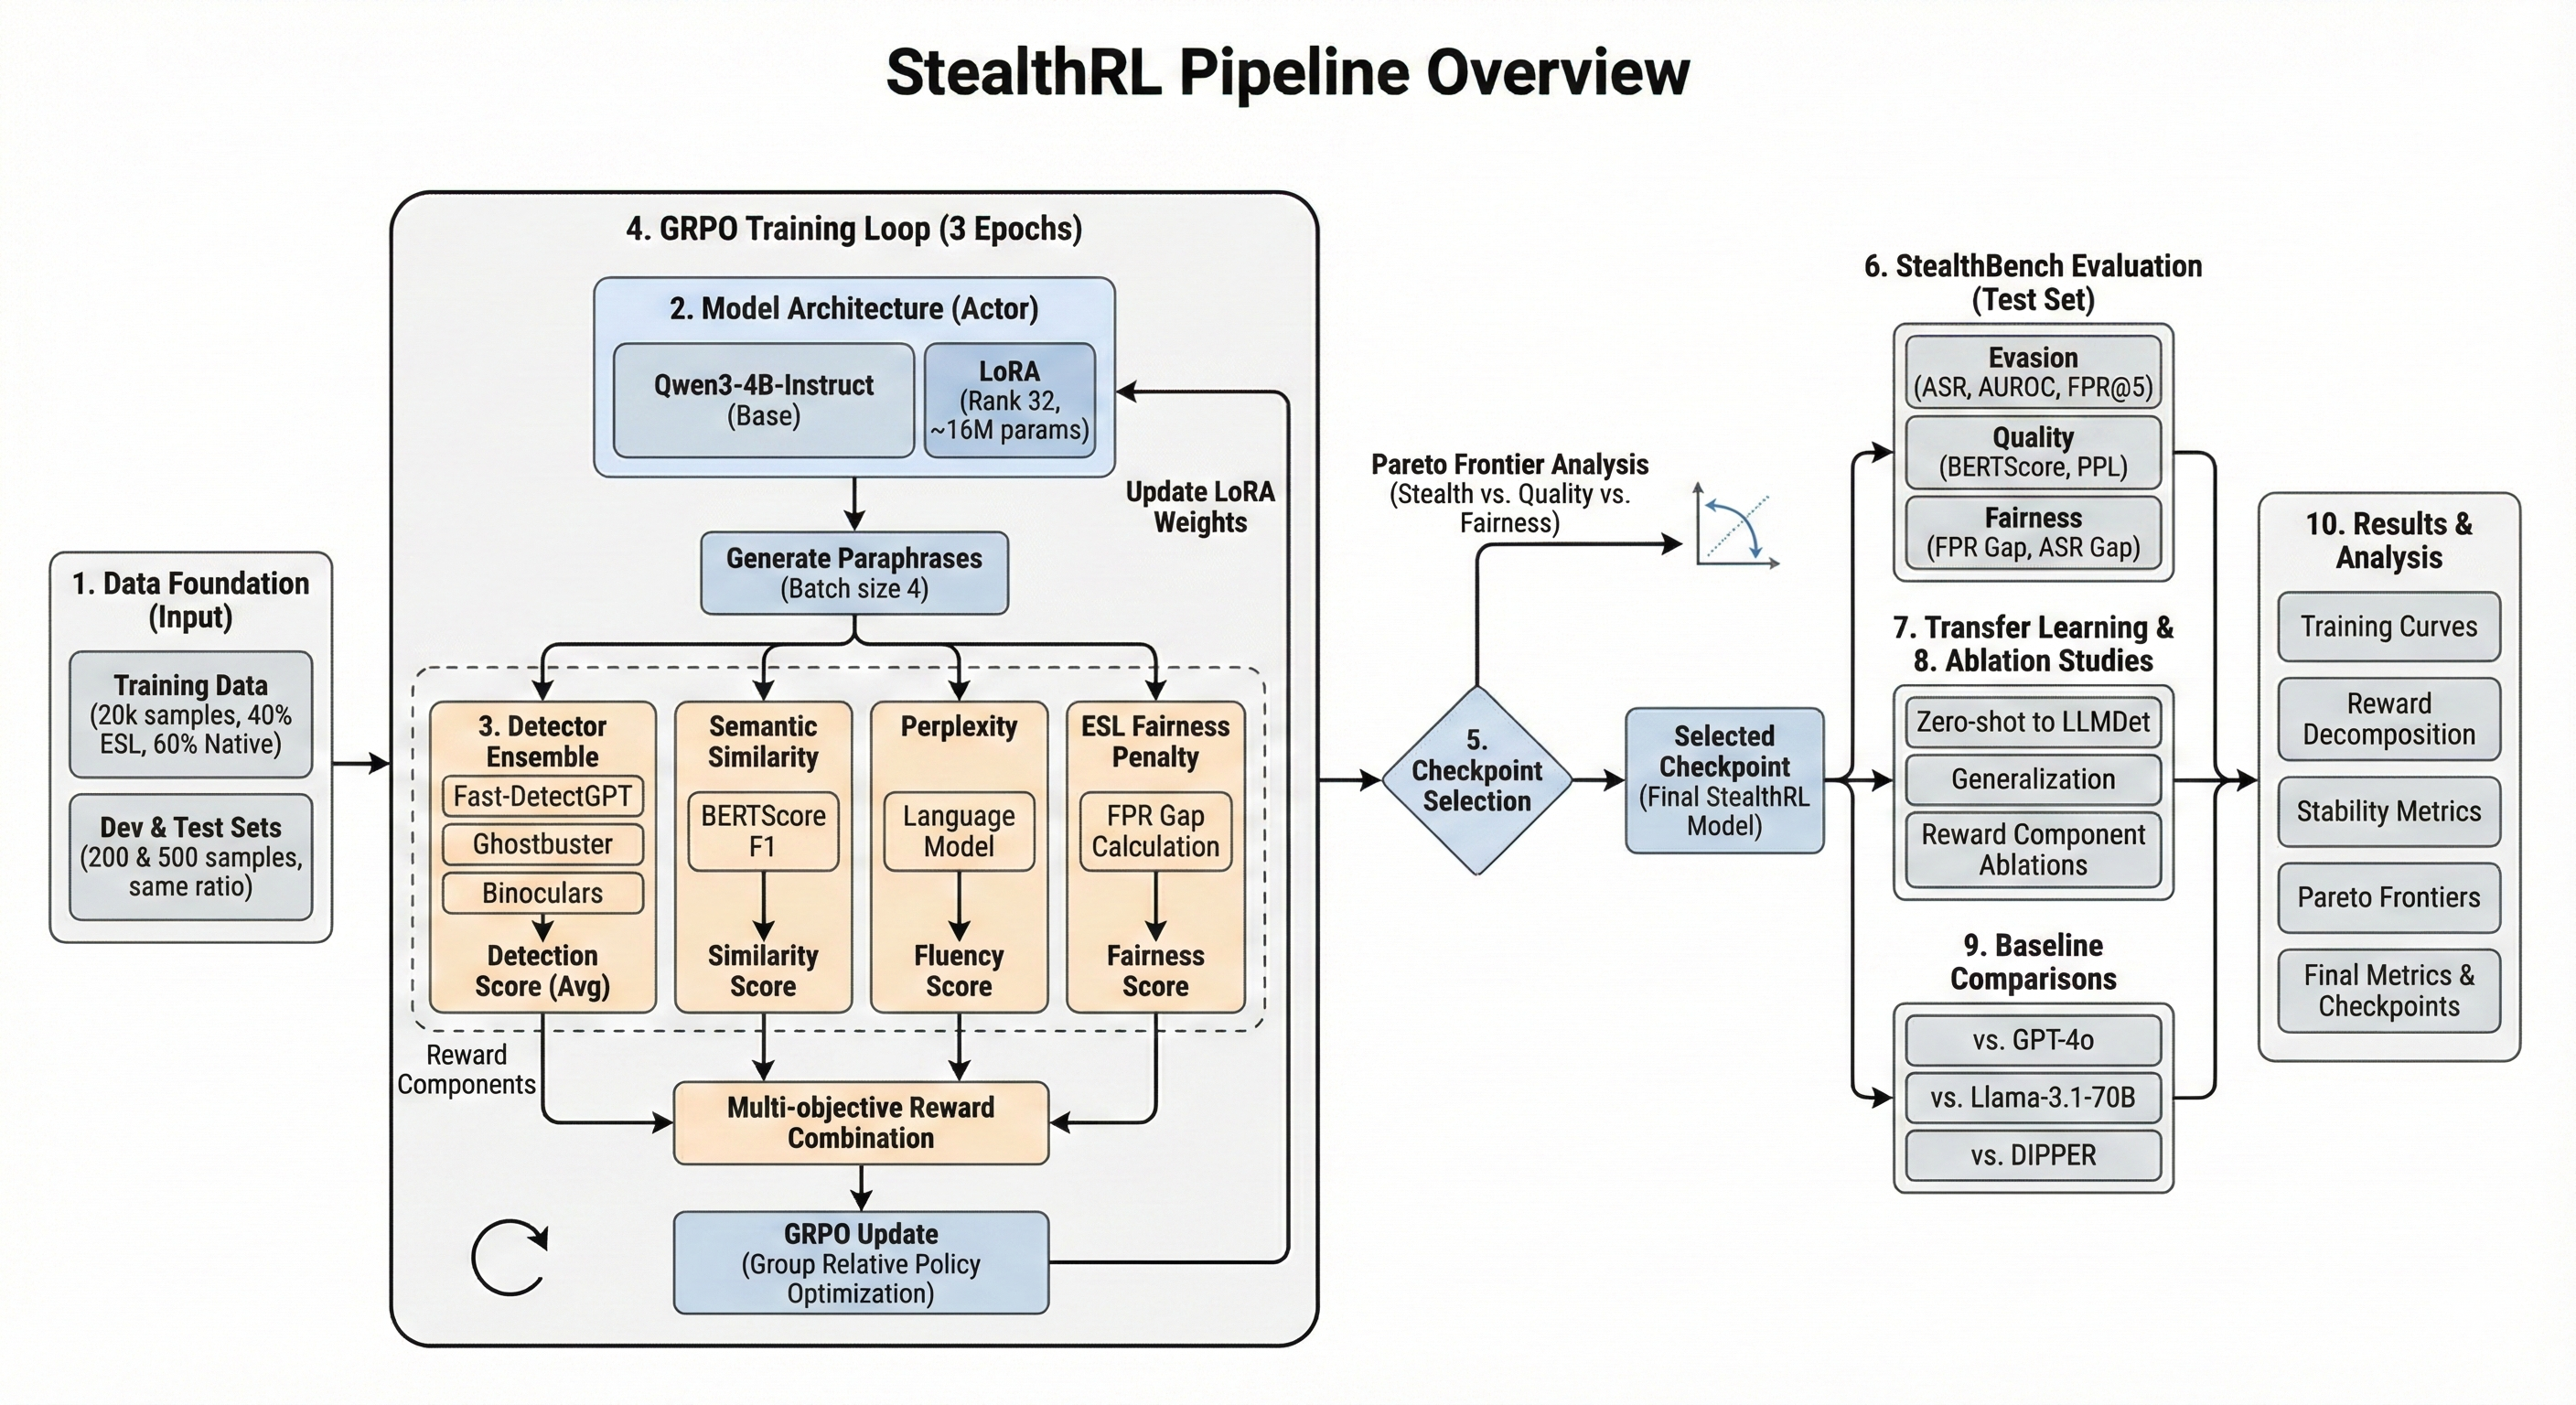
\includegraphics[width=\textwidth]{StealthRL_Methodology.png}
\caption{StealthRL pipeline overview showing the complete training loop from data foundation through GRPO optimization, checkpoint selection, and comprehensive evaluation including fairness, transfer learning, and baseline comparisons.}
\label{fig:architecture}
\end{figure}

\section{Results}
\textbf{Proof-of-concept.} We validate stability and trade-offs in an ultra-fast configuration (800 examples; single-detector reward using Fast-DetectGPT). The best checkpoint reduces Fast-DetectGPT detection probability from 0.587 to 0.458 while maintaining high semantic similarity (avg 0.986). Training remains stable with parse success improving from 0.859 to 0.992 and KL divergence staying below 0.4.

\begin{table}[t]
\centering
\small
\begin{tabular}{lccc}
\toprule
Metric & Initial & Best checkpoint & Final \\
\midrule
Detector probability (Fast-DetectGPT) $\downarrow$ & 0.587 & 0.458 & 0.579 \\
Semantic similarity (cosine) $\uparrow$ & 0.986 & 0.944 & 0.987 \\
Parse success $\uparrow$ & 0.859 & 1.000 & 0.992 \\
KL divergence $\downarrow$ & 0.01 & 0.25 & 0.25 \\
\bottomrule
\end{tabular}
\caption{StealthRL proof-of-concept metrics (800 samples; single-detector feedback).}
\label{tab:poc}
\end{table}

\begin{figure}[t]
\centering
\includegraphics[width=0.85\textwidth]{pareto_frontiers.png}
\caption{Pareto frontier analysis showing trade-offs between stealth (detector evasion), quality (semantic similarity), and fairness (ESL disparity reduction) across training checkpoints.}
\label{fig:pareto}
\end{figure}

\textbf{Multi-detector and fairness evaluation (ongoing).} The full-scale experiment is currently running with ensemble training over heterogeneous detector families (curvature-based, classifier-based, paired-LM) and ESL-balanced evaluation that reports disparity metrics under low-FPR operating points. We are conducting multiple ablation studies to isolate the contributions of each reward component and to quantify transfer across detector types. These results will be ready to present by the symposium date.

\section{Amazon Nova evaluation track}
To align with the symposium emphasis on Amazon Nova, StealthRL includes a Bedrock-based evaluation track that will use Amazon Nova models as follows:
\begin{itemize}
  \item \textbf{Robustness stratification by source model:} generate base texts with Amazon Nova and compare detector behavior across sources under matched prompts and lengths.
  \item \textbf{Optional semantic judging:} use a Nova model as a secondary semantic faithfulness judge to confirm that paraphrases preserve meaning, complementing embedding-based similarity.
\end{itemize}
This track is model-agnostic and will use the symposium-provided Nova credits to produce reproducible evaluation artifacts suitable for detector calibration and monitoring.

\section{Conclusion}
StealthRL provides a practical post-training framework for Trusted AI evaluation of AI-text detectors. It combines RL with fidelity, fluency, and ESL-aware regularization to generate controlled paraphrases that surface robustness gaps and help quantify disparity. Our proof-of-concept results show meaningful detector-confidence reduction with high semantic preservation and stable training, and our Nova-enabled evaluation track supports broader, model-agnostic assessment aligned with the symposium priorities.

\small\bibliographystyle{plainnat}\begin{thebibliography}{9}

\bibitem{mitchell2023detectgpt}
E. Mitchell, Y. Lee, A. Khazatsky, C. D. Manning, and C. Finn.
DetectGPT: Zero-shot machine-generated text detection using probability curvature.
\emph{ICML}, 2023.

\bibitem{bao2024fastdetect}
G. Bao et al.
Fast-DetectGPT: Efficient zero-shot detection of machine-generated text via conditional probability curvature.
\emph{ICLR}, 2024.

\bibitem{verma2024ghostbuster}
V. Verma et al.
Ghostbuster: Detecting text ghostwritten by large language models.
\emph{NAACL}, 2024.

\bibitem{hans2024binoculars}
A. Hans et al.
Spotting LLMs with Binoculars: Zero-shot detection of machine-generated text.
\emph{ICML}, 2024.

\bibitem{liang2023bias}
Weixin Liang, et al.
GPT detectors are biased against non-native English writers.
\emph{Patterns}, 4(7), 2023.

\bibitem{david2025authormist}
Idan David and Arthur Gervais.
AuthorMist: Evading AI text detectors with reinforcement learning.
arXiv:2503.08716, 2025.

\bibitem{lu2024sico}
Jiaqi Lu, et al.
SICO: Substitution-based in-context optimization for evading AI text detectors.
arXiv:2402.04636, 2024.

\bibitem{hu2022lora}
E. J. Hu et al.
LoRA: Low-rank adaptation of large language models.
\emph{ICLR}, 2022.
See also: \url{https://thinkingmachines.ai/blog/lora/}.

\bibitem{awsnova}
AWS Documentation.
Amazon Nova User Guide and model specifications (Amazon Bedrock).
\url{https://docs.aws.amazon.com/nova/latest/userguide/what-is-nova.html}.

\end{thebibliography}

\end{document}